\documentclass[11pt]{article}

    \usepackage[breakable]{tcolorbox}
    \usepackage{parskip} % Stop auto-indenting (to mimic markdown behaviour)
    

    % Basic figure setup, for now with no caption control since it's done
    % automatically by Pandoc (which extracts ![](path) syntax from Markdown).
    \usepackage{graphicx}
    % Maintain compatibility with old templates. Remove in nbconvert 6.0
    \let\Oldincludegraphics\includegraphics
    % Ensure that by default, figures have no caption (until we provide a
    % proper Figure object with a Caption API and a way to capture that
    % in the conversion process - todo).
    \usepackage{caption}
    \DeclareCaptionFormat{nocaption}{}
    \captionsetup{format=nocaption,aboveskip=0pt,belowskip=0pt}

    \usepackage{float}
    \floatplacement{figure}{H} % forces figures to be placed at the correct location
    \usepackage{xcolor} % Allow colors to be defined
    \usepackage{enumerate} % Needed for markdown enumerations to work
    \usepackage{geometry} % Used to adjust the document margins
    \usepackage{amsmath} % Equations
    \usepackage{amssymb} % Equations
    \usepackage{textcomp} % defines textquotesingle
    % Hack from http://tex.stackexchange.com/a/47451/13684:
    \AtBeginDocument{%
        \def\PYZsq{\textquotesingle}% Upright quotes in Pygmentized code
    }
    \usepackage{upquote} % Upright quotes for verbatim code
    \usepackage{eurosym} % defines \euro

    \usepackage{iftex}
    \ifPDFTeX
        \usepackage[T1]{fontenc}
        \IfFileExists{alphabeta.sty}{
              \usepackage{alphabeta}
          }{
              \usepackage[mathletters]{ucs}
              \usepackage[utf8x]{inputenc}
          }
    \else
        \usepackage{fontspec}
        \usepackage{unicode-math}
    \fi

    \usepackage{fancyvrb} % verbatim replacement that allows latex
    \usepackage{grffile} % extends the file name processing of package graphics 
                         % to support a larger range
    \makeatletter % fix for old versions of grffile with XeLaTeX
    \@ifpackagelater{grffile}{2019/11/01}
    {
      % Do nothing on new versions
    }
    {
      \def\Gread@@xetex#1{%
        \IfFileExists{"\Gin@base".bb}%
        {\Gread@eps{\Gin@base.bb}}%
        {\Gread@@xetex@aux#1}%
      }
    }
    \makeatother
    \usepackage[Export]{adjustbox} % Used to constrain images to a maximum size
    \adjustboxset{max size={0.9\linewidth}{0.9\paperheight}}

    % The hyperref package gives us a pdf with properly built
    % internal navigation ('pdf bookmarks' for the table of contents,
    % internal cross-reference links, web links for URLs, etc.)
    \usepackage{hyperref}
    % The default LaTeX title has an obnoxious amount of whitespace. By default,
    % titling removes some of it. It also provides customization options.
    \usepackage{titling}
    \usepackage{longtable} % longtable support required by pandoc >1.10
    \usepackage{booktabs}  % table support for pandoc > 1.12.2
    \usepackage{array}     % table support for pandoc >= 2.11.3
    \usepackage{calc}      % table minipage width calculation for pandoc >= 2.11.1
    \usepackage[inline]{enumitem} % IRkernel/repr support (it uses the enumerate* environment)
    \usepackage[normalem]{ulem} % ulem is needed to support strikethroughs (\sout)
                                % normalem makes italics be italics, not underlines
    \usepackage{mathrsfs}
    

    
    % Colors for the hyperref package
    \definecolor{urlcolor}{rgb}{0,.145,.698}
    \definecolor{linkcolor}{rgb}{.71,0.21,0.01}
    \definecolor{citecolor}{rgb}{.12,.54,.11}

    % ANSI colors
    \definecolor{ansi-black}{HTML}{3E424D}
    \definecolor{ansi-black-intense}{HTML}{282C36}
    \definecolor{ansi-red}{HTML}{E75C58}
    \definecolor{ansi-red-intense}{HTML}{B22B31}
    \definecolor{ansi-green}{HTML}{00A250}
    \definecolor{ansi-green-intense}{HTML}{007427}
    \definecolor{ansi-yellow}{HTML}{DDB62B}
    \definecolor{ansi-yellow-intense}{HTML}{B27D12}
    \definecolor{ansi-blue}{HTML}{208FFB}
    \definecolor{ansi-blue-intense}{HTML}{0065CA}
    \definecolor{ansi-magenta}{HTML}{D160C4}
    \definecolor{ansi-magenta-intense}{HTML}{A03196}
    \definecolor{ansi-cyan}{HTML}{60C6C8}
    \definecolor{ansi-cyan-intense}{HTML}{258F8F}
    \definecolor{ansi-white}{HTML}{C5C1B4}
    \definecolor{ansi-white-intense}{HTML}{A1A6B2}
    \definecolor{ansi-default-inverse-fg}{HTML}{FFFFFF}
    \definecolor{ansi-default-inverse-bg}{HTML}{000000}

    % common color for the border for error outputs.
    \definecolor{outerrorbackground}{HTML}{FFDFDF}

    % commands and environments needed by pandoc snippets
    % extracted from the output of `pandoc -s`
    \providecommand{\tightlist}{%
      \setlength{\itemsep}{0pt}\setlength{\parskip}{0pt}}
    \DefineVerbatimEnvironment{Highlighting}{Verbatim}{commandchars=\\\{\}}
    % Add ',fontsize=\small' for more characters per line
    \newenvironment{Shaded}{}{}
    \newcommand{\KeywordTok}[1]{\textcolor[rgb]{0.00,0.44,0.13}{\textbf{{#1}}}}
    \newcommand{\DataTypeTok}[1]{\textcolor[rgb]{0.56,0.13,0.00}{{#1}}}
    \newcommand{\DecValTok}[1]{\textcolor[rgb]{0.25,0.63,0.44}{{#1}}}
    \newcommand{\BaseNTok}[1]{\textcolor[rgb]{0.25,0.63,0.44}{{#1}}}
    \newcommand{\FloatTok}[1]{\textcolor[rgb]{0.25,0.63,0.44}{{#1}}}
    \newcommand{\CharTok}[1]{\textcolor[rgb]{0.25,0.44,0.63}{{#1}}}
    \newcommand{\StringTok}[1]{\textcolor[rgb]{0.25,0.44,0.63}{{#1}}}
    \newcommand{\CommentTok}[1]{\textcolor[rgb]{0.38,0.63,0.69}{\textit{{#1}}}}
    \newcommand{\OtherTok}[1]{\textcolor[rgb]{0.00,0.44,0.13}{{#1}}}
    \newcommand{\AlertTok}[1]{\textcolor[rgb]{1.00,0.00,0.00}{\textbf{{#1}}}}
    \newcommand{\FunctionTok}[1]{\textcolor[rgb]{0.02,0.16,0.49}{{#1}}}
    \newcommand{\RegionMarkerTok}[1]{{#1}}
    \newcommand{\ErrorTok}[1]{\textcolor[rgb]{1.00,0.00,0.00}{\textbf{{#1}}}}
    \newcommand{\NormalTok}[1]{{#1}}
    
    % Additional commands for more recent versions of Pandoc
    \newcommand{\ConstantTok}[1]{\textcolor[rgb]{0.53,0.00,0.00}{{#1}}}
    \newcommand{\SpecialCharTok}[1]{\textcolor[rgb]{0.25,0.44,0.63}{{#1}}}
    \newcommand{\VerbatimStringTok}[1]{\textcolor[rgb]{0.25,0.44,0.63}{{#1}}}
    \newcommand{\SpecialStringTok}[1]{\textcolor[rgb]{0.73,0.40,0.53}{{#1}}}
    \newcommand{\ImportTok}[1]{{#1}}
    \newcommand{\DocumentationTok}[1]{\textcolor[rgb]{0.73,0.13,0.13}{\textit{{#1}}}}
    \newcommand{\AnnotationTok}[1]{\textcolor[rgb]{0.38,0.63,0.69}{\textbf{\textit{{#1}}}}}
    \newcommand{\CommentVarTok}[1]{\textcolor[rgb]{0.38,0.63,0.69}{\textbf{\textit{{#1}}}}}
    \newcommand{\VariableTok}[1]{\textcolor[rgb]{0.10,0.09,0.49}{{#1}}}
    \newcommand{\ControlFlowTok}[1]{\textcolor[rgb]{0.00,0.44,0.13}{\textbf{{#1}}}}
    \newcommand{\OperatorTok}[1]{\textcolor[rgb]{0.40,0.40,0.40}{{#1}}}
    \newcommand{\BuiltInTok}[1]{{#1}}
    \newcommand{\ExtensionTok}[1]{{#1}}
    \newcommand{\PreprocessorTok}[1]{\textcolor[rgb]{0.74,0.48,0.00}{{#1}}}
    \newcommand{\AttributeTok}[1]{\textcolor[rgb]{0.49,0.56,0.16}{{#1}}}
    \newcommand{\InformationTok}[1]{\textcolor[rgb]{0.38,0.63,0.69}{\textbf{\textit{{#1}}}}}
    \newcommand{\WarningTok}[1]{\textcolor[rgb]{0.38,0.63,0.69}{\textbf{\textit{{#1}}}}}
    
    
    % Define a nice break command that doesn't care if a line doesn't already
    % exist.
    \def\br{\hspace*{\fill} \\* }
    % Math Jax compatibility definitions
    \def\gt{>}
    \def\lt{<}
    \let\Oldtex\TeX
    \let\Oldlatex\LaTeX
    \renewcommand{\TeX}{\textrm{\Oldtex}}
    \renewcommand{\LaTeX}{\textrm{\Oldlatex}}
    % Document parameters
    % Document title
    \title{Plain\_Ryan\_HW1\_report}
    
    
    
    
    
% Pygments definitions
\makeatletter
\def\PY@reset{\let\PY@it=\relax \let\PY@bf=\relax%
    \let\PY@ul=\relax \let\PY@tc=\relax%
    \let\PY@bc=\relax \let\PY@ff=\relax}
\def\PY@tok#1{\csname PY@tok@#1\endcsname}
\def\PY@toks#1+{\ifx\relax#1\empty\else%
    \PY@tok{#1}\expandafter\PY@toks\fi}
\def\PY@do#1{\PY@bc{\PY@tc{\PY@ul{%
    \PY@it{\PY@bf{\PY@ff{#1}}}}}}}
\def\PY#1#2{\PY@reset\PY@toks#1+\relax+\PY@do{#2}}

\@namedef{PY@tok@w}{\def\PY@tc##1{\textcolor[rgb]{0.73,0.73,0.73}{##1}}}
\@namedef{PY@tok@c}{\let\PY@it=\textit\def\PY@tc##1{\textcolor[rgb]{0.25,0.50,0.50}{##1}}}
\@namedef{PY@tok@cp}{\def\PY@tc##1{\textcolor[rgb]{0.74,0.48,0.00}{##1}}}
\@namedef{PY@tok@k}{\let\PY@bf=\textbf\def\PY@tc##1{\textcolor[rgb]{0.00,0.50,0.00}{##1}}}
\@namedef{PY@tok@kp}{\def\PY@tc##1{\textcolor[rgb]{0.00,0.50,0.00}{##1}}}
\@namedef{PY@tok@kt}{\def\PY@tc##1{\textcolor[rgb]{0.69,0.00,0.25}{##1}}}
\@namedef{PY@tok@o}{\def\PY@tc##1{\textcolor[rgb]{0.40,0.40,0.40}{##1}}}
\@namedef{PY@tok@ow}{\let\PY@bf=\textbf\def\PY@tc##1{\textcolor[rgb]{0.67,0.13,1.00}{##1}}}
\@namedef{PY@tok@nb}{\def\PY@tc##1{\textcolor[rgb]{0.00,0.50,0.00}{##1}}}
\@namedef{PY@tok@nf}{\def\PY@tc##1{\textcolor[rgb]{0.00,0.00,1.00}{##1}}}
\@namedef{PY@tok@nc}{\let\PY@bf=\textbf\def\PY@tc##1{\textcolor[rgb]{0.00,0.00,1.00}{##1}}}
\@namedef{PY@tok@nn}{\let\PY@bf=\textbf\def\PY@tc##1{\textcolor[rgb]{0.00,0.00,1.00}{##1}}}
\@namedef{PY@tok@ne}{\let\PY@bf=\textbf\def\PY@tc##1{\textcolor[rgb]{0.82,0.25,0.23}{##1}}}
\@namedef{PY@tok@nv}{\def\PY@tc##1{\textcolor[rgb]{0.10,0.09,0.49}{##1}}}
\@namedef{PY@tok@no}{\def\PY@tc##1{\textcolor[rgb]{0.53,0.00,0.00}{##1}}}
\@namedef{PY@tok@nl}{\def\PY@tc##1{\textcolor[rgb]{0.63,0.63,0.00}{##1}}}
\@namedef{PY@tok@ni}{\let\PY@bf=\textbf\def\PY@tc##1{\textcolor[rgb]{0.60,0.60,0.60}{##1}}}
\@namedef{PY@tok@na}{\def\PY@tc##1{\textcolor[rgb]{0.49,0.56,0.16}{##1}}}
\@namedef{PY@tok@nt}{\let\PY@bf=\textbf\def\PY@tc##1{\textcolor[rgb]{0.00,0.50,0.00}{##1}}}
\@namedef{PY@tok@nd}{\def\PY@tc##1{\textcolor[rgb]{0.67,0.13,1.00}{##1}}}
\@namedef{PY@tok@s}{\def\PY@tc##1{\textcolor[rgb]{0.73,0.13,0.13}{##1}}}
\@namedef{PY@tok@sd}{\let\PY@it=\textit\def\PY@tc##1{\textcolor[rgb]{0.73,0.13,0.13}{##1}}}
\@namedef{PY@tok@si}{\let\PY@bf=\textbf\def\PY@tc##1{\textcolor[rgb]{0.73,0.40,0.53}{##1}}}
\@namedef{PY@tok@se}{\let\PY@bf=\textbf\def\PY@tc##1{\textcolor[rgb]{0.73,0.40,0.13}{##1}}}
\@namedef{PY@tok@sr}{\def\PY@tc##1{\textcolor[rgb]{0.73,0.40,0.53}{##1}}}
\@namedef{PY@tok@ss}{\def\PY@tc##1{\textcolor[rgb]{0.10,0.09,0.49}{##1}}}
\@namedef{PY@tok@sx}{\def\PY@tc##1{\textcolor[rgb]{0.00,0.50,0.00}{##1}}}
\@namedef{PY@tok@m}{\def\PY@tc##1{\textcolor[rgb]{0.40,0.40,0.40}{##1}}}
\@namedef{PY@tok@gh}{\let\PY@bf=\textbf\def\PY@tc##1{\textcolor[rgb]{0.00,0.00,0.50}{##1}}}
\@namedef{PY@tok@gu}{\let\PY@bf=\textbf\def\PY@tc##1{\textcolor[rgb]{0.50,0.00,0.50}{##1}}}
\@namedef{PY@tok@gd}{\def\PY@tc##1{\textcolor[rgb]{0.63,0.00,0.00}{##1}}}
\@namedef{PY@tok@gi}{\def\PY@tc##1{\textcolor[rgb]{0.00,0.63,0.00}{##1}}}
\@namedef{PY@tok@gr}{\def\PY@tc##1{\textcolor[rgb]{1.00,0.00,0.00}{##1}}}
\@namedef{PY@tok@ge}{\let\PY@it=\textit}
\@namedef{PY@tok@gs}{\let\PY@bf=\textbf}
\@namedef{PY@tok@gp}{\let\PY@bf=\textbf\def\PY@tc##1{\textcolor[rgb]{0.00,0.00,0.50}{##1}}}
\@namedef{PY@tok@go}{\def\PY@tc##1{\textcolor[rgb]{0.53,0.53,0.53}{##1}}}
\@namedef{PY@tok@gt}{\def\PY@tc##1{\textcolor[rgb]{0.00,0.27,0.87}{##1}}}
\@namedef{PY@tok@err}{\def\PY@bc##1{{\setlength{\fboxsep}{\string -\fboxrule}\fcolorbox[rgb]{1.00,0.00,0.00}{1,1,1}{\strut ##1}}}}
\@namedef{PY@tok@kc}{\let\PY@bf=\textbf\def\PY@tc##1{\textcolor[rgb]{0.00,0.50,0.00}{##1}}}
\@namedef{PY@tok@kd}{\let\PY@bf=\textbf\def\PY@tc##1{\textcolor[rgb]{0.00,0.50,0.00}{##1}}}
\@namedef{PY@tok@kn}{\let\PY@bf=\textbf\def\PY@tc##1{\textcolor[rgb]{0.00,0.50,0.00}{##1}}}
\@namedef{PY@tok@kr}{\let\PY@bf=\textbf\def\PY@tc##1{\textcolor[rgb]{0.00,0.50,0.00}{##1}}}
\@namedef{PY@tok@bp}{\def\PY@tc##1{\textcolor[rgb]{0.00,0.50,0.00}{##1}}}
\@namedef{PY@tok@fm}{\def\PY@tc##1{\textcolor[rgb]{0.00,0.00,1.00}{##1}}}
\@namedef{PY@tok@vc}{\def\PY@tc##1{\textcolor[rgb]{0.10,0.09,0.49}{##1}}}
\@namedef{PY@tok@vg}{\def\PY@tc##1{\textcolor[rgb]{0.10,0.09,0.49}{##1}}}
\@namedef{PY@tok@vi}{\def\PY@tc##1{\textcolor[rgb]{0.10,0.09,0.49}{##1}}}
\@namedef{PY@tok@vm}{\def\PY@tc##1{\textcolor[rgb]{0.10,0.09,0.49}{##1}}}
\@namedef{PY@tok@sa}{\def\PY@tc##1{\textcolor[rgb]{0.73,0.13,0.13}{##1}}}
\@namedef{PY@tok@sb}{\def\PY@tc##1{\textcolor[rgb]{0.73,0.13,0.13}{##1}}}
\@namedef{PY@tok@sc}{\def\PY@tc##1{\textcolor[rgb]{0.73,0.13,0.13}{##1}}}
\@namedef{PY@tok@dl}{\def\PY@tc##1{\textcolor[rgb]{0.73,0.13,0.13}{##1}}}
\@namedef{PY@tok@s2}{\def\PY@tc##1{\textcolor[rgb]{0.73,0.13,0.13}{##1}}}
\@namedef{PY@tok@sh}{\def\PY@tc##1{\textcolor[rgb]{0.73,0.13,0.13}{##1}}}
\@namedef{PY@tok@s1}{\def\PY@tc##1{\textcolor[rgb]{0.73,0.13,0.13}{##1}}}
\@namedef{PY@tok@mb}{\def\PY@tc##1{\textcolor[rgb]{0.40,0.40,0.40}{##1}}}
\@namedef{PY@tok@mf}{\def\PY@tc##1{\textcolor[rgb]{0.40,0.40,0.40}{##1}}}
\@namedef{PY@tok@mh}{\def\PY@tc##1{\textcolor[rgb]{0.40,0.40,0.40}{##1}}}
\@namedef{PY@tok@mi}{\def\PY@tc##1{\textcolor[rgb]{0.40,0.40,0.40}{##1}}}
\@namedef{PY@tok@il}{\def\PY@tc##1{\textcolor[rgb]{0.40,0.40,0.40}{##1}}}
\@namedef{PY@tok@mo}{\def\PY@tc##1{\textcolor[rgb]{0.40,0.40,0.40}{##1}}}
\@namedef{PY@tok@ch}{\let\PY@it=\textit\def\PY@tc##1{\textcolor[rgb]{0.25,0.50,0.50}{##1}}}
\@namedef{PY@tok@cm}{\let\PY@it=\textit\def\PY@tc##1{\textcolor[rgb]{0.25,0.50,0.50}{##1}}}
\@namedef{PY@tok@cpf}{\let\PY@it=\textit\def\PY@tc##1{\textcolor[rgb]{0.25,0.50,0.50}{##1}}}
\@namedef{PY@tok@c1}{\let\PY@it=\textit\def\PY@tc##1{\textcolor[rgb]{0.25,0.50,0.50}{##1}}}
\@namedef{PY@tok@cs}{\let\PY@it=\textit\def\PY@tc##1{\textcolor[rgb]{0.25,0.50,0.50}{##1}}}

\def\PYZbs{\char`\\}
\def\PYZus{\char`\_}
\def\PYZob{\char`\{}
\def\PYZcb{\char`\}}
\def\PYZca{\char`\^}
\def\PYZam{\char`\&}
\def\PYZlt{\char`\<}
\def\PYZgt{\char`\>}
\def\PYZsh{\char`\#}
\def\PYZpc{\char`\%}
\def\PYZdl{\char`\$}
\def\PYZhy{\char`\-}
\def\PYZsq{\char`\'}
\def\PYZdq{\char`\"}
\def\PYZti{\char`\~}
% for compatibility with earlier versions
\def\PYZat{@}
\def\PYZlb{[}
\def\PYZrb{]}
\makeatother


    % For linebreaks inside Verbatim environment from package fancyvrb. 
    \makeatletter
        \newbox\Wrappedcontinuationbox 
        \newbox\Wrappedvisiblespacebox 
        \newcommand*\Wrappedvisiblespace {\textcolor{red}{\textvisiblespace}} 
        \newcommand*\Wrappedcontinuationsymbol {\textcolor{red}{\llap{\tiny$\m@th\hookrightarrow$}}} 
        \newcommand*\Wrappedcontinuationindent {3ex } 
        \newcommand*\Wrappedafterbreak {\kern\Wrappedcontinuationindent\copy\Wrappedcontinuationbox} 
        % Take advantage of the already applied Pygments mark-up to insert 
        % potential linebreaks for TeX processing. 
        %        {, <, #, %, $, ' and ": go to next line. 
        %        _, }, ^, &, >, - and ~: stay at end of broken line. 
        % Use of \textquotesingle for straight quote. 
        \newcommand*\Wrappedbreaksatspecials {% 
            \def\PYGZus{\discretionary{\char`\_}{\Wrappedafterbreak}{\char`\_}}% 
            \def\PYGZob{\discretionary{}{\Wrappedafterbreak\char`\{}{\char`\{}}% 
            \def\PYGZcb{\discretionary{\char`\}}{\Wrappedafterbreak}{\char`\}}}% 
            \def\PYGZca{\discretionary{\char`\^}{\Wrappedafterbreak}{\char`\^}}% 
            \def\PYGZam{\discretionary{\char`\&}{\Wrappedafterbreak}{\char`\&}}% 
            \def\PYGZlt{\discretionary{}{\Wrappedafterbreak\char`\<}{\char`\<}}% 
            \def\PYGZgt{\discretionary{\char`\>}{\Wrappedafterbreak}{\char`\>}}% 
            \def\PYGZsh{\discretionary{}{\Wrappedafterbreak\char`\#}{\char`\#}}% 
            \def\PYGZpc{\discretionary{}{\Wrappedafterbreak\char`\%}{\char`\%}}% 
            \def\PYGZdl{\discretionary{}{\Wrappedafterbreak\char`\$}{\char`\$}}% 
            \def\PYGZhy{\discretionary{\char`\-}{\Wrappedafterbreak}{\char`\-}}% 
            \def\PYGZsq{\discretionary{}{\Wrappedafterbreak\textquotesingle}{\textquotesingle}}% 
            \def\PYGZdq{\discretionary{}{\Wrappedafterbreak\char`\"}{\char`\"}}% 
            \def\PYGZti{\discretionary{\char`\~}{\Wrappedafterbreak}{\char`\~}}% 
        } 
        % Some characters . , ; ? ! / are not pygmentized. 
        % This macro makes them "active" and they will insert potential linebreaks 
        \newcommand*\Wrappedbreaksatpunct {% 
            \lccode`\~`\.\lowercase{\def~}{\discretionary{\hbox{\char`\.}}{\Wrappedafterbreak}{\hbox{\char`\.}}}% 
            \lccode`\~`\,\lowercase{\def~}{\discretionary{\hbox{\char`\,}}{\Wrappedafterbreak}{\hbox{\char`\,}}}% 
            \lccode`\~`\;\lowercase{\def~}{\discretionary{\hbox{\char`\;}}{\Wrappedafterbreak}{\hbox{\char`\;}}}% 
            \lccode`\~`\:\lowercase{\def~}{\discretionary{\hbox{\char`\:}}{\Wrappedafterbreak}{\hbox{\char`\:}}}% 
            \lccode`\~`\?\lowercase{\def~}{\discretionary{\hbox{\char`\?}}{\Wrappedafterbreak}{\hbox{\char`\?}}}% 
            \lccode`\~`\!\lowercase{\def~}{\discretionary{\hbox{\char`\!}}{\Wrappedafterbreak}{\hbox{\char`\!}}}% 
            \lccode`\~`\/\lowercase{\def~}{\discretionary{\hbox{\char`\/}}{\Wrappedafterbreak}{\hbox{\char`\/}}}% 
            \catcode`\.\active
            \catcode`\,\active 
            \catcode`\;\active
            \catcode`\:\active
            \catcode`\?\active
            \catcode`\!\active
            \catcode`\/\active 
            \lccode`\~`\~ 	
        }
    \makeatother

    \let\OriginalVerbatim=\Verbatim
    \makeatletter
    \renewcommand{\Verbatim}[1][1]{%
        %\parskip\z@skip
        \sbox\Wrappedcontinuationbox {\Wrappedcontinuationsymbol}%
        \sbox\Wrappedvisiblespacebox {\FV@SetupFont\Wrappedvisiblespace}%
        \def\FancyVerbFormatLine ##1{\hsize\linewidth
            \vtop{\raggedright\hyphenpenalty\z@\exhyphenpenalty\z@
                \doublehyphendemerits\z@\finalhyphendemerits\z@
                \strut ##1\strut}%
        }%
        % If the linebreak is at a space, the latter will be displayed as visible
        % space at end of first line, and a continuation symbol starts next line.
        % Stretch/shrink are however usually zero for typewriter font.
        \def\FV@Space {%
            \nobreak\hskip\z@ plus\fontdimen3\font minus\fontdimen4\font
            \discretionary{\copy\Wrappedvisiblespacebox}{\Wrappedafterbreak}
            {\kern\fontdimen2\font}%
        }%
        
        % Allow breaks at special characters using \PYG... macros.
        \Wrappedbreaksatspecials
        % Breaks at punctuation characters . , ; ? ! and / need catcode=\active 	
        \OriginalVerbatim[#1,codes*=\Wrappedbreaksatpunct]%
    }
    \makeatother

    % Exact colors from NB
    \definecolor{incolor}{HTML}{303F9F}
    \definecolor{outcolor}{HTML}{D84315}
    \definecolor{cellborder}{HTML}{CFCFCF}
    \definecolor{cellbackground}{HTML}{F7F7F7}
    
    % prompt
    \makeatletter
    \newcommand{\boxspacing}{\kern\kvtcb@left@rule\kern\kvtcb@boxsep}
    \makeatother
    \newcommand{\prompt}[4]{
        {\ttfamily\llap{{\color{#2}[#3]:\hspace{3pt}#4}}\vspace{-\baselineskip}}
    }
    

    
    % Prevent overflowing lines due to hard-to-break entities
    \sloppy 
    % Setup hyperref package
    \hypersetup{
      breaklinks=true,  % so long urls are correctly broken across lines
      colorlinks=true,
      urlcolor=urlcolor,
      linkcolor=linkcolor,
      citecolor=citecolor,
      }
    % Slightly bigger margins than the latex defaults
    
    \geometry{verbose,tmargin=1in,bmargin=1in,lmargin=1in,rmargin=1in}
    
    

\begin{document}
    
    \maketitle
    
    

    
    \hypertarget{homework-1}{%
\section{Homework 1}\label{homework-1}}

    \hypertarget{concept-questions}{%
\subsection{1.) Concept Questions}\label{concept-questions}}

\hypertarget{whats-the-main-difference-between-supervised-and-unsupervised-learning}{%
\paragraph{1.) What's the main difference between supervised and
unsupervised
learning?}\label{whats-the-main-difference-between-supervised-and-unsupervised-learning}}

The main difference between supervised and unsupervised learning is
having the labels of the training data prior to modeling. In supervised
learning, you would be classifying a test data set after training on
data that was already labeled or classified. Unsupervised learning, such
as k-means, would be learning the clusters or classifications from
unlabeled data. Unsupervised learning also can call for adding
subjectivity or domain knowledge into the analysis to make sense of the
output.

\hypertarget{will-different-initializations-for-k-means-lead-to-different-results}{%
\paragraph{2.) Will different initializations for k-means lead to
different
results?}\label{will-different-initializations-for-k-means-lead-to-different-results}}

Yes, due to the fact that it is a non-convex optimization problem. This
could lead to multiple local solutions and we would only end up in one
of them. Depending on the starting point, if there are multiple local
solutions you could end up at different solutions based on
initializaiton. This also means that it is not guarenteed to find the
global minimal optimization solutions.

\hypertarget{give-a-short-proof-can-be-in-words-but-using-correct-logic-why-k-means-algorithm-will-converge-in-finite-number-of-iterations.}{%
\paragraph{3.) Give a short proof (can be in words but using correct
logic) why k-means algorithm will converge in finite number of
iterations.}\label{give-a-short-proof-can-be-in-words-but-using-correct-logic-why-k-means-algorithm-will-converge-in-finite-number-of-iterations.}}

Since there are a fixed number of data points, there are only a finite
number of combinations to calculate the centroids. The algorithm will
try to reduce a certain metric, and you can continue to decrease until
it is not able to decrease any further. This could take many iterations,
but eventually it will always converge.

\hypertarget{what-is-the-main-difference-between-k-means-and-generalized-k-means-algorithm-explain-how-the-choice-of-the-similaritydissimilaritydistance-will-impact-the-result.}{%
\paragraph{4.) What is the main difference between k-means and
generalized k-means algorithm? Explain how the choice of the
similarity/dissimilarity/distance will impact the
result.}\label{what-is-the-main-difference-between-k-means-and-generalized-k-means-algorithm-explain-how-the-choice-of-the-similaritydissimilaritydistance-will-impact-the-result.}}

The differnce everything to do with the similarity measure. K-means uses
Euclidean distance, where the generalized k-means algorithm can use any
similarity measure. Replacing the Euclidean distance with a general
definition can allow it to be a convex optimization problem. This also
allows customization for different types of datasets where Euclidian is
not the best solution for the objective.

\hypertarget{write-down-the-graph-laplacian-matrix-and-find-the-eigenvectors-associated-with-the-zero-eigen--value.-explain-how-do-you-find-out-the-number-of-disconnected-clusters-in-graph-and-identify-these-disconnected-clusters-using-these-eigenvectors.}{%
\paragraph{5.) Write down the graph Laplacian matrix and find the
eigenvectors associated with the zero eigen- value. Explain how do you
find out the number of disconnected clusters in graph and identify these
disconnected clusters using these
eigenvectors.}\label{write-down-the-graph-laplacian-matrix-and-find-the-eigenvectors-associated-with-the-zero-eigen--value.-explain-how-do-you-find-out-the-number-of-disconnected-clusters-in-graph-and-identify-these-disconnected-clusters-using-these-eigenvectors.}}

    \begin{tcolorbox}[breakable, size=fbox, boxrule=1pt, pad at break*=1mm,colback=cellbackground, colframe=cellborder]
\prompt{In}{incolor}{19}{\boxspacing}
\begin{Verbatim}[commandchars=\\\{\}]
\PY{n}{A} \PY{o}{=} \PY{n}{np}\PY{o}{.}\PY{n}{array}\PY{p}{(}\PY{p}{[}
    \PY{p}{[}\PY{l+m+mi}{0}\PY{p}{,} \PY{l+m+mi}{1}\PY{p}{,} \PY{l+m+mi}{1}\PY{p}{,} \PY{l+m+mi}{0}\PY{p}{,} \PY{l+m+mi}{0}\PY{p}{]}\PY{p}{,}
    \PY{p}{[}\PY{l+m+mi}{1}\PY{p}{,} \PY{l+m+mi}{0}\PY{p}{,} \PY{l+m+mi}{1}\PY{p}{,} \PY{l+m+mi}{0}\PY{p}{,} \PY{l+m+mi}{0}\PY{p}{]}\PY{p}{,}
    \PY{p}{[}\PY{l+m+mi}{1}\PY{p}{,} \PY{l+m+mi}{1}\PY{p}{,} \PY{l+m+mi}{0}\PY{p}{,} \PY{l+m+mi}{0}\PY{p}{,} \PY{l+m+mi}{0}\PY{p}{]}\PY{p}{,}
    \PY{p}{[}\PY{l+m+mi}{0}\PY{p}{,} \PY{l+m+mi}{0}\PY{p}{,} \PY{l+m+mi}{0}\PY{p}{,} \PY{l+m+mi}{0}\PY{p}{,} \PY{l+m+mi}{1}\PY{p}{]}\PY{p}{,}
    \PY{p}{[}\PY{l+m+mi}{0}\PY{p}{,} \PY{l+m+mi}{0}\PY{p}{,} \PY{l+m+mi}{0}\PY{p}{,} \PY{l+m+mi}{1}\PY{p}{,} \PY{l+m+mi}{0}\PY{p}{]}
    \PY{p}{]}\PY{p}{)}

\PY{n}{D} \PY{o}{=} \PY{n}{np}\PY{o}{.}\PY{n}{array}\PY{p}{(}\PY{p}{[}
    \PY{p}{[}\PY{l+m+mi}{2}\PY{p}{,} \PY{l+m+mi}{0}\PY{p}{,} \PY{l+m+mi}{0}\PY{p}{,} \PY{l+m+mi}{0}\PY{p}{,} \PY{l+m+mi}{0}\PY{p}{]}\PY{p}{,}
    \PY{p}{[}\PY{l+m+mi}{0}\PY{p}{,} \PY{l+m+mi}{2}\PY{p}{,} \PY{l+m+mi}{0}\PY{p}{,} \PY{l+m+mi}{0}\PY{p}{,} \PY{l+m+mi}{0}\PY{p}{]}\PY{p}{,}
    \PY{p}{[}\PY{l+m+mi}{0}\PY{p}{,} \PY{l+m+mi}{0}\PY{p}{,} \PY{l+m+mi}{2}\PY{p}{,} \PY{l+m+mi}{0}\PY{p}{,} \PY{l+m+mi}{0}\PY{p}{]}\PY{p}{,}
    \PY{p}{[}\PY{l+m+mi}{0}\PY{p}{,} \PY{l+m+mi}{0}\PY{p}{,} \PY{l+m+mi}{0}\PY{p}{,} \PY{l+m+mi}{1}\PY{p}{,} \PY{l+m+mi}{0}\PY{p}{]}\PY{p}{,}
    \PY{p}{[}\PY{l+m+mi}{0}\PY{p}{,} \PY{l+m+mi}{0}\PY{p}{,} \PY{l+m+mi}{0}\PY{p}{,} \PY{l+m+mi}{0}\PY{p}{,} \PY{l+m+mi}{1}\PY{p}{]}
\PY{p}{]}\PY{p}{)}

\PY{n}{L} \PY{o}{=} \PY{n}{D} \PY{o}{\PYZhy{}} \PY{n}{A}
\PY{n}{L}
\end{Verbatim}
\end{tcolorbox}

            \begin{tcolorbox}[breakable, size=fbox, boxrule=.5pt, pad at break*=1mm, opacityfill=0]
\prompt{Out}{outcolor}{19}{\boxspacing}
\begin{Verbatim}[commandchars=\\\{\}]
array([[ 2, -1, -1,  0,  0],
       [-1,  2, -1,  0,  0],
       [-1, -1,  2,  0,  0],
       [ 0,  0,  0,  1, -1],
       [ 0,  0,  0, -1,  1]])
\end{Verbatim}
\end{tcolorbox}
        
    \begin{tcolorbox}[breakable, size=fbox, boxrule=1pt, pad at break*=1mm,colback=cellbackground, colframe=cellborder]
\prompt{In}{incolor}{20}{\boxspacing}
\begin{Verbatim}[commandchars=\\\{\}]
\PY{n}{U}\PY{p}{,} \PY{n}{V} \PY{o}{=} \PY{n}{np}\PY{o}{.}\PY{n}{linalg}\PY{o}{.}\PY{n}{eig}\PY{p}{(}\PY{n}{L}\PY{p}{)}
\end{Verbatim}
\end{tcolorbox}

    \hypertarget{eigenvectors}{%
\subparagraph{Eigenvectors}\label{eigenvectors}}

    \begin{tcolorbox}[breakable, size=fbox, boxrule=1pt, pad at break*=1mm,colback=cellbackground, colframe=cellborder]
\prompt{In}{incolor}{21}{\boxspacing}
\begin{Verbatim}[commandchars=\\\{\}]
\PY{n}{V}
\end{Verbatim}
\end{tcolorbox}

            \begin{tcolorbox}[breakable, size=fbox, boxrule=.5pt, pad at break*=1mm, opacityfill=0]
\prompt{Out}{outcolor}{21}{\boxspacing}
\begin{Verbatim}[commandchars=\\\{\}]
array([[ 0.81649658, -0.57735027,  0.30959441,  0.        ,  0.        ],
       [-0.40824829, -0.57735027, -0.80910101,  0.        ,  0.        ],
       [-0.40824829, -0.57735027,  0.49950661,  0.        ,  0.        ],
       [ 0.        ,  0.        ,  0.        ,  0.70710678,  0.70710678],
       [ 0.        ,  0.        ,  0.        , -0.70710678,  0.70710678]])
\end{Verbatim}
\end{tcolorbox}
        
    \hypertarget{eigenvalues}{%
\subparagraph{Eigenvalues}\label{eigenvalues}}

    \begin{tcolorbox}[breakable, size=fbox, boxrule=1pt, pad at break*=1mm,colback=cellbackground, colframe=cellborder]
\prompt{In}{incolor}{22}{\boxspacing}
\begin{Verbatim}[commandchars=\\\{\}]
\PY{n}{U}
\end{Verbatim}
\end{tcolorbox}

            \begin{tcolorbox}[breakable, size=fbox, boxrule=.5pt, pad at break*=1mm, opacityfill=0]
\prompt{Out}{outcolor}{22}{\boxspacing}
\begin{Verbatim}[commandchars=\\\{\}]
array([ 3.00000000e+00, -3.77809194e-16,  3.00000000e+00,  2.00000000e+00,
        0.00000000e+00])
\end{Verbatim}
\end{tcolorbox}
        
    \hypertarget{identifying-the-clusters}{%
\subparagraph{Identifying the clusters}\label{identifying-the-clusters}}

To find the clusters from the eigenvectors, the eigenvectors with
eigenvalue 0 contain cluster assignment information.The rows that have
similar eigenvectors are from similar communities, and clustered
together.

    \begin{center}\rule{0.5\linewidth}{0.5pt}\end{center}

\hypertarget{image-compression-using-clustering}{%
\subsection{2.) Image compression using
clustering}\label{image-compression-using-clustering}}

    \hypertarget{euclidean}{%
\paragraph{1.) Euclidean}\label{euclidean}}

Utilizing the Kmeans cluster algorithm, I was able to create image
compressions by clustering the individual pixels of the image. Each
image begins with randomized centorids bassed on the \(k\) clusters
passed to the method. It then iterates assigning each row to the closest
centorid based on the \(L2\) distance. The centroids are then updated by
taking the average of each cluster group. This continues until
convergence where the centroids no longer change (stopping when the
centorids are less than 0.001 in difference than the previous
iteration).

For the analysis, each image was ran 5 times per cluster, on
\(k = [2, 4, 6, 8, 16]\).

As the number of clusters increased, the iterations and time it took to
converge also increased. For the Football image, lower \(k\) completed
in an average of 11 to 18 seconds, where higher \(k\) finished around 40
seconds. The variance was much higher as you increase \(k\). Depending
on the randomized centroids, the solution could converge quickly, or it
could take quite a while relative to other runs due to poor starting
points. It is possible to select the exact sample pixel (not point, but
same pixel elsewhere in the image) and that would cause an error with
the algorthim. To handle this, if the number of unique initilized
centroids did not equal \(k\), they were re-initilized until that held
true.

The Georgia Tech image had interesting results. For \(k = 2\), it
converged quickly with minimal variance. For \(k = 4\), it still
converged quickly in an average of 22 iterations, but the variance was
133. I don't believe it is a property internal to the image, but it does
show that centroid selection to begin can have a large affect on the
model run time.

I then ran the algorithm on two other images, of my cat and child. The
image of the baby was notable because the variance was much higher for
\(k=8\) than that of \(k=16\). They did not seem to be as complex as the
provided images, converging much faster than the other 2.

Outputs of the images below. The higher the \(k\), the more pixelated
the image. It depends on the tradeoff you are looking for as to which
works best for you. If this was to input thousands of images into a
model, it might be better to use a lower \(k\), and capture the rough
outlines.

\(k = 6\) 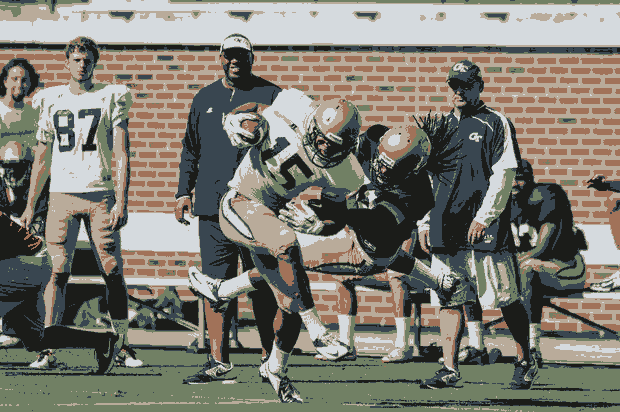
\includegraphics{img/football_6_cluster_euclidean.png}

\(k = 16\) 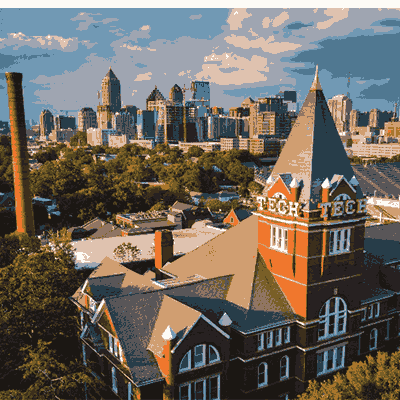
\includegraphics{img/GeorgiaTech_16_cluster_euclidean.png}

\(k = 6\) 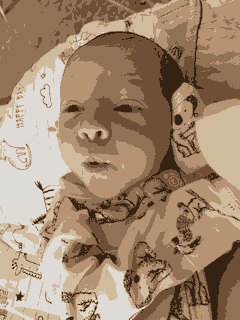
\includegraphics{img/IMG_1401_6_cluster_euclidean.png}

\(k = 4\) 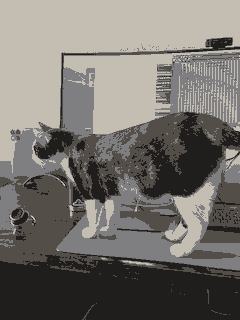
\includegraphics{img/cat_4_euclidean.png}

\hypertarget{manhattan}{%
\paragraph{2.) Manhattan}\label{manhattan}}

The next part of the analysis was replicating the algorithm, except this
time using the Manhattan distance. This would be taking the \(L1\) norm,
where the distance is calculated by taking the sum of length of the
\(Y\) axis direction and \(X\) axis direction. Manhattan is the nickname
due to it's similarity of a taxi driving through blocks in Manhattan.
Centroids were updated using the median values for each iteration.

By using the Manhattan distance, there was an increase in the time it
took to converge relative to the Euclidean distance for the Football,
Baby, and Cat images. However, the Georgia Tech image converged quicker
with Manhatten.

\(k = 16\) 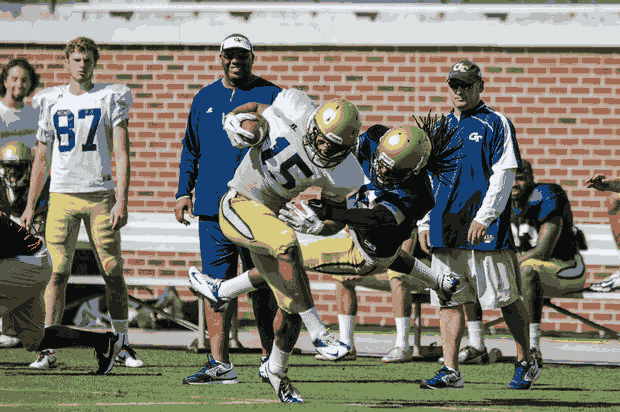
\includegraphics{img/football_16_cluster_cityblock.png}

\(k = 4\) 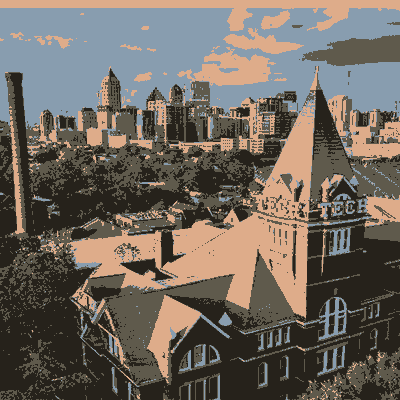
\includegraphics{img/GeorgiaTech_4_cluster_cityblock.png}

    \begin{tcolorbox}[breakable, size=fbox, boxrule=1pt, pad at break*=1mm,colback=cellbackground, colframe=cellborder]
\prompt{In}{incolor}{ }{\boxspacing}
\begin{Verbatim}[commandchars=\\\{\}]

\end{Verbatim}
\end{tcolorbox}


    % Add a bibliography block to the postdoc
    
    
    
\end{document}
